% ------------------------------------------------------------------------ %
% !TEX encoding = UTF-8 Unicode
% !TEX TS-program = pdflatex
% !TEX root = ../Tesi.tex
% !TEX spellcheck = it-IT
% ------------------------------------------------------------------------ %
%
% ------------------------------------------------------------------------ %
% 	CAD Deployment

\chapter[CAD Deployment for Indoor WSNs]{Towards Smart Building Design Automation: CAD Deployment for Indoor WSNs}
\label{cap:cad}


\section{Introduction}
\label{sec:CADintro}
As described in chapter \ref{cap:soa}, over the last years many smart buildings applications have been subject of intense research.
Smart environments usually rely on several hardware nodes equipped with sensors, actuators and communication functionalities.
A clear example is the occupancy monitoring system presented in chapter \ref{cap:bluesentinel}, but the same applies for different applications like indoor localization or safety systems.\\
The high level of heterogeneity and the lack of standardization across technologies make design of such environments a very challenging task, as each installation has to be designed manually and performed ad-hoc for the specific building.
On the other hand, many different systems show common characteristics, like the strict dependency with the building floor plan, also sharing similar requirements such as a nodes allocation that provides sensing coverage and nodes connectivity.

The work explained in this chapter consists in a CAD application for the design of smart building systems based on the installation of hardware nodes across the indoor space. The tool provides a site-specific algorithm for cost-effective deployment of wireless localization systems, with the aim to maximize the localization accuracy.

%Experimental results from real-world environment show that the proposed site-specific model can improve the positioning accuracy of general models from the \mbox{state-of-the-art}.
The tool, born to assist the installation of the BlueSentinel system, has become general-purpose and extensible through plug-ins allowing to model building systems with different requirements.
The results of this project have been presented at UBICOMP 2016 \cite{Cirigliano2016} and will be published in TCAD (Transactions on Computer-Aided Design of Integrated Circuits and Systems).

\section{The Nodes Deployment Problem}
\label{sec:deploy-problem}

Many smart buildings applications are based on indoor localization techniques, using location information to optimize the environment and provide context-aware services.\\
Indoor localization systems often require the presence of wireless devices such as Access Points (AP), in order to let the user identify its position by means of a mobile device.\\
Most smart building applications have been developed in order to achieve sustainability, reducing energy waste related to energy-consuming appliances like Heating, Ventilation, and Air-Conditioning (HVAC). Some examples are \cite{Erickson2011} and \cite{Balaji2013}. Smart HVAC systems usually rely on a set of ambient sensors able to collect indoor values of temperature and humidity. This allows the control system to build thermal maps of the indoor environment, locate thermal complaint feedbacks coming from the tenants and regulate only the necessary portion of the physical system.\\
Another target feature of complex buildings is safety, characterized by the ability to respond to crisis events limiting damages and victims. These systems are able to detect safety threats, for example from smoke detectors or heat detectors. Also in this scenario, a proper allocation of sensor nodes is essential to detect and locate the threat responsively.

\smallskip
The position of each node strongly affects the performance of the system, since a bad allocation could lead to unmonitored areas.
%encumber: gravare; sinonimi: burden, weigh (pesare figurato).
The number of nodes employed, besides weighting on the installation cost, also burdens the overall energy consumption of the system, a key parameter to consider especially for energy saving systems.\\
The choice of the hardware nodes can get more difficult by the availability on the market of several devices and components that differ in cost, power consumption and maximum range distance.

\smallskip
Although the key role of nodes allocation, many smart building systems proposed in literature don't consider nodes amount and positioning problems in environments that differ from the original testbeds.\\
Without a systematic approach the design space is not well explored, which leads to inefficient solutions.
In this context, the development of tools able to automatize part of the design flow of smart building systems is essential.
In order to find a near-optimal allocation of nodes, the knowledge of the floor plan is required. However, for installations performed on existing buildings, administrators can encounter difficulties in obtaining the floor plan in an easily-interpretable digital format.
%recupero floorplan, posizionamento, costo totale / accuratezza, installazione è costosa, tuning / spostamento è unfeasible

To address these problems, we developed a CAD tool to assist building designers during the design of smart building systems.
The application manages common requirements like the building floor plan specification. We decided to implement a node allocation algorithm for three different indoor localization systems, that searches for  near-optimal 
%aiming to keep low ...
allocations of nodes, from mixed hardware types, with the aim of keeping low the total cost. Due to the high level of heterogeneity and lack of standardization across systems to design, we make the system extensible through plug-ins to let new functionalities being integrated into the system.
The tool\footnote{A video demo of the tool has been published at \url{https://youtu.be/5BnFU9iXXWo}}
is developed within the QCAD\footnote{QCAD - Open Source CAD System: \url{http://www.qcad.org/}} environment, an \mbox{open-source} computer-aided drafting application. The key contributions of our work can be summarized in the following:
\begin{itemize}
\item A traditional CAD interface to specify both the physical building floor-plan and the functional components of the smart environment.
\item An algorithm for hardware nodes allocation that provides to designers a near-optimal placement of devices. The algorithm explores combinations of different types of nodes to obtain cost-effective solutions.
\item A site-specific model for wireless indoor localization accuracy optimization that keeps into account the actual structure of the building.
\item The integration of the tool within an \mbox{open-source}\footnote{The source code of the system is \mbox{open-source} and available at \url{https://bitbucket.org/necst/box-smartcad}} application framework able to extend the system by means of JavaScript or C++ plug-ins.
\end{itemize}

\section{Related Work}\label{sec:related}
Building Information Modeling (BIM) is a consolidate process to support building constructions and renovations. BIM softwares, and in particular CAD for buildings such as ArchiCAD~\cite{Archicad}, focus on the generation and management of digital representations of the physical aspects of places. BIM tools can coordinate architectural and structural requirements, for essential tasks such as collision detection~\cite{Zhang2011}. Materials employed for a construction can be represented with extremely high levels of accuracy, thanks to the several libraries developed in many years, resulting in precise cost estimations~\cite{Xu2014}. With the diffusion of integrated smart systems built to increase comfort and efficiency, buildings require the design of aspects that go beyond the mere physical design. The concept of smart environment is becoming more and more concrete with the integration of sensors, actuators and computational elements in buildings, while tools able to model smart and interactive functionalities of modern buildings are currently lacking.

The problem of the allocation of hardware nodes in a given environment can be compared, on first approximation, by the maximal cover location problem (MCLP), i.e. the problem of covering the maximum amount of demand locations with a given number of facilities. Similarly, the location set covering problem (LSCP) consists in finding the minimum set of facilities that covers all available demand locations. Each facility has the same coverage radius \(r\); a demand point is assumed to be covered if it is within distance \(r\) of a facility. Daskin et al. gave a general formulation of the LSCP \cite{Daskin1983} and re-formulated it for network systems and emergency vehicle deployment \cite{Daskin1981}.

The maximum sensing coverage region (MSCR) is a special case of the previous two problems that focuses on the research of an allocation of wireless nodes that guarantees both sensing coverage and network connectivity between nodes~\cite{VinhTranQuang, So2005}. In this scenario the placement need to take care not only of the sensing range, but also of the communication range of each node.
%Questi approcci citati hanno lo svantaggio di considerare le singole locazioni come variabili binarie coperte/scoperte, senza modellizzare le performance complessive del sistema.

\begin{table}
\centering
\def\arraystretch{1}
\label{tab:comparison}
\caption{Comparison between proposed deployment methods and tools for indoor WSN and Access Points based systems.}
\begin{tabulary}{\textwidth}{| L | L | L | L | L |}
    \hline
    \textbf{Deployment} & \textbf{Site Specific vs General Model} & \textbf{Heterogeneous Nodes} & \textbf{Application Integrated} & \textbf{Extensible} \\ \hline
    Zhao et al. \cite{Zhao2008} & General Model & No & Yes & No\\ \hline
    He at al. \cite{He2011} & General Model & No & No & No\\ \hline
    Fang et. al. \cite{Fang2010} & Site Specific Model & No & No & No\\ \hline
    Proposed approach & Site Specific Model & Yes & Yes & Yes\\ \hline

    \end{tabulary}
\end{table}

For what concern the allocation in indoor environments, only minimum literature has been published so far to the best of our knowledge. Zhao et al. in \cite{Zhao2008} proposed an access point (AP) positioning model based on the Differential Evolution algorithm, specific for fingerprinting localization techniques. Their model focuses on increasing the diversity of the received signal array along the indoor locations, and thus improving the positioning accuracy of fingerprinting schemes.
However, the model does not take into account the effect of walls or other obstacles present in the target environment.
%However, the model is not suitable for triangulation and sensing monitoring positioning problems.
%In addition, the model does not take into account the effect of walls, doors and other obstacles.
He at al. in \cite{He2011} made use of a genetic algorithm for APs deployment model, to study the relationship between positioning error and signal space Euclidean distance. Again, the simulation results show that the error can be reduced increasing the Euclidean distance between the RSS (Received Signal Strength) arrays of different locations.
%This has been achieved increasing the number of APs until a certain range, but the results show that ``the more the better'' rule does not necessarily hold.
%Similarly to the previous work, the authors used a simple signal propagation approach and did not consider the attenuation effects of the indoor environment.
Fang et. al. in \cite{Fang2010} proposed a tool for linking the placement of APs and the positioning performance. Their algorithm maximizes signal-to-noise ratio (SNR) i.e. maximizes the signal and minimizes the noise simultaneously. However, the system is developed in a real-world environment, and requires measurements with different access point allocations that can be an expensive and time-consuming task.

A common limitation of many works described previously is the employment of simple and general models which doesn't take into account the actual layout and geometry of the building. The free-space path loss propagation model is often used despite the presence of fixed obstructing objects like walls. Of course, none of the cited works provide a convenient way to specify geometric layout of the indoor environment. This leads the authors to validate models simply using squared or rectangular areas to represent the indoor environment, omitting the relationship between irregular areas and system coverage.
%The result can lead designers in time-consuming maps configuration, and error-prone design phase for the allocation of hardware nodes.
In addition, none of the existing solutions takes in consideration different hardware characteristics and costs of the nodes to be deployed.

\section{The Proposed Application Framework}\label{sec:components}
Our system has been developed on top of the QCAD application framework. The QCAD Application Framework consists of programming libraries and resources that provides CAD specific functionalities. An example of module provided by the QCAD Application framework is the Math module that implements mathematical concepts such as vectors or matrices as well as basic geometrical classes like points, lines and so on. The QCAD Framework has been enhanced with a \emph{SmartBuilding} module that provides some fundamental functionalities for the design of smart building systems. The module include abstract entities like rooms, walls, sockets, sensor nodes and gateways. User interface components are also provided in order to create and edit this entities (\emph{tools}) and to specify parameters (\emph{widgets}). Our module implements a node deployment algorithm for three commons indoor localization systems, that will be discussed later.
The whole application rely on Qt, a framework that covers a lot of generic and low level functionality for desktop applications and not directly related to CAD.
\begin{figure}[h!tb]
\centering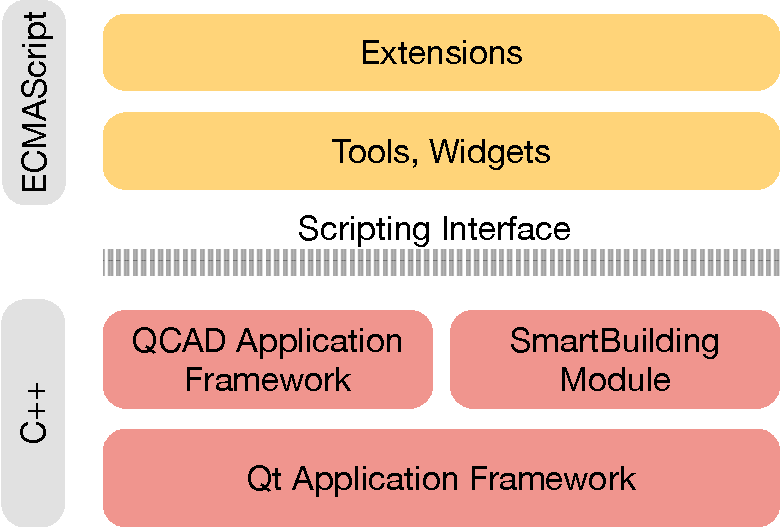
\includegraphics[scale=0.7]{framework.pdf}
\caption[Overview of the CAD application framework stack.]{Overview of the application stack. The script interpreter features standard ECMAScript functionality and on top of that provides additional classes from the Qt API, QCAD API and the \emph{SmartBuilding} module.}
\end{figure}

The QCAD Application Framework offers a very complete and powerful ECMAScript interface. The SmartBuilding module, as well as the QCAD Application Framework, is accessible through that scripting interface. Through the ECMAScript interface developers will be able to extend the whole application in an easy and very efficient way. The choice of a popular script language that is easy to learn enables anyone with previous programming experience to extend the application. Such extensions can for example be CAD related interactive tools like an HVAC layout construction widget, or a temperature sensor nodes deployment algorithm.
%piazzamento sens temp humi, 
%or user interface components (widgets).

In some situations extending QCAD through scripts alone may not be possible. This is mostly the case, if the extension is based on an existing C or C++ library. In that case, it is possible to create a C++ plug-in that wraps the existing library and adds the necessary hooks to access library functionality through the script interface. Such a plug-in will be automatically loaded by QCAD on start up to add functions and classes to the script interface of QCAD. These script extensions can then be used by a script add-ons to make that functionality available as part of the application interface.


\begin{figure}[h!tb]
\centering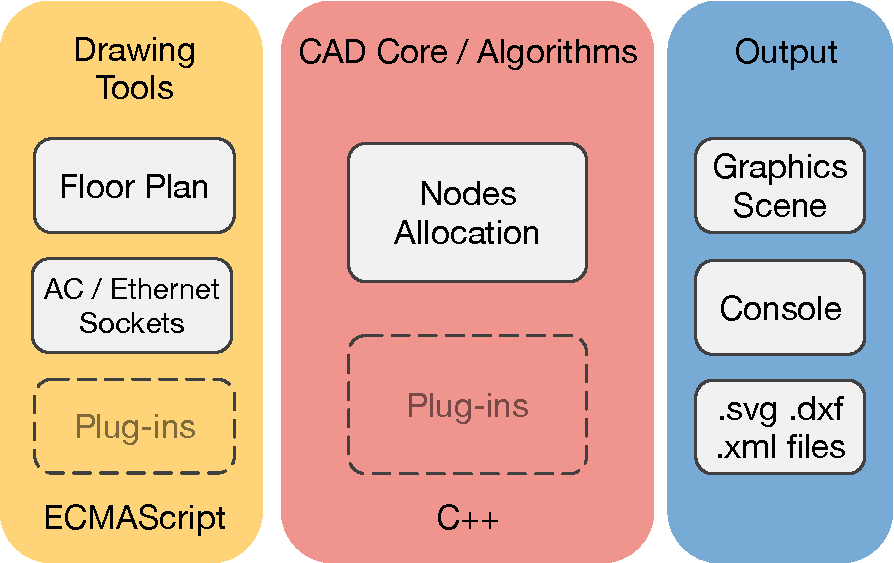
\includegraphics[scale=0.7]{extend.pdf}
\caption[Functional overview of the system components of the CAD application.]{Functional overview of the system components. Drawing tools and algorithms for systems deployment and simulation are extensible through ECMAScript or C++ plug-ins.}
\end{figure}

\begin{figure}
\centering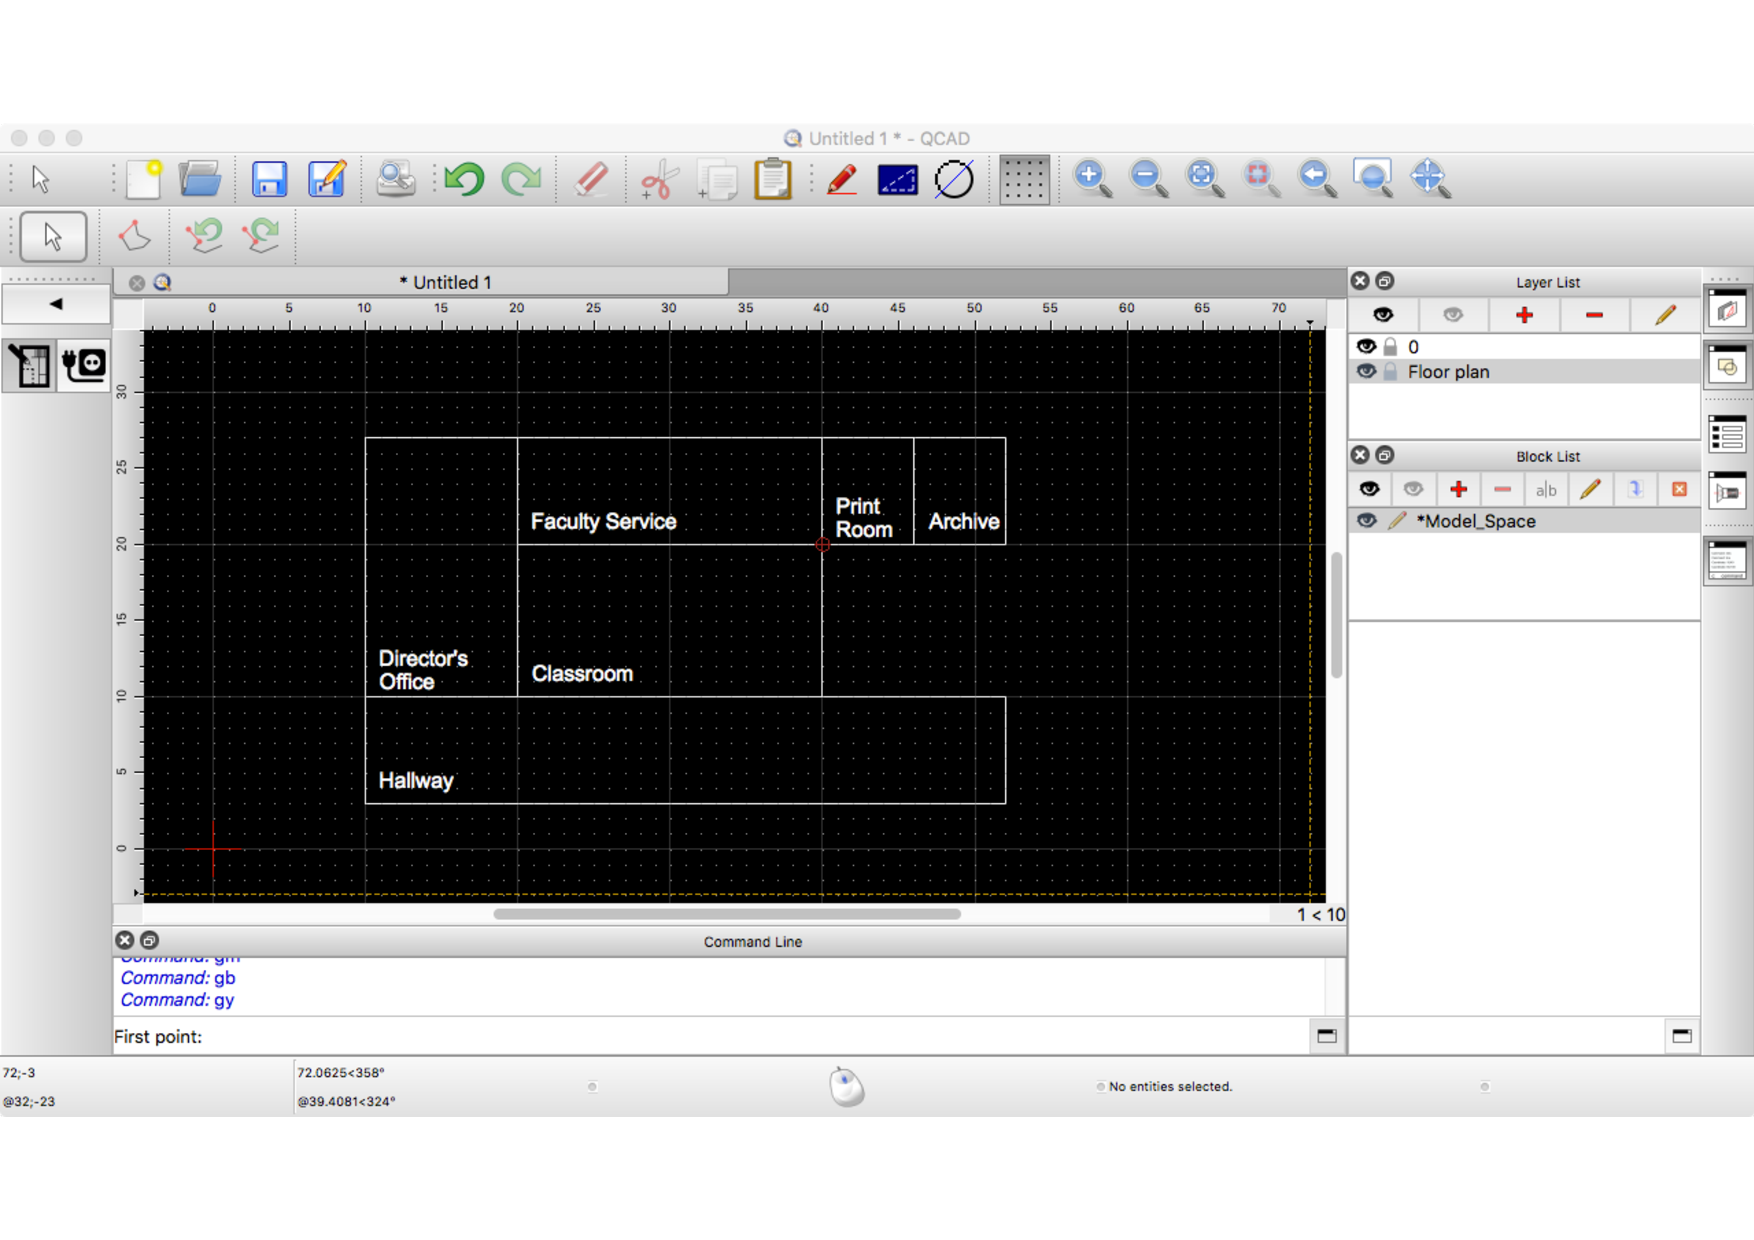
\includegraphics[width=\linewidth]{floorplan2.pdf}
\caption[Graphical interface of the floor-plan design of the CAD tool.]{Floor-plan design tool. User can specify the layout of the rooms and a possible set of candidate sites for the node placement.}
\label{fig:floor}
\end{figure}

\section{Nodes Deployment for Indoor Localization}\label{sec:problem}
Smart environments always rely on a set of hardware nodes able to collect sensing data and communicate through cabled or wireless technologies. The number of nodes employed and the position of each one strongly affect the overall performance of the system as well as the cost of installation.
In our work, indoor localization systems have been taken as the main case study for the nodes allocation, since occupants localization and monitoring is one of the most common requirements of different smart environments.

The way in which the indoor environment must be covered by the nodes depends on the particular technology implemented, however there can be identified three main manners: 
\begin{enumerate}[label={(\arabic*)}]
\item Single Coverage, i.e. to monitor the state of the environment with a single node for each location inside its radius. This includes for example to detect the presence of a mobile device in a proximity region \cite{Andersson2014}, or to detect a RFID tag within the tags reader range \cite{Paul2014}.
\item Trilateration, to compute the position of a mobile device. This technique requires the reception of a wireless signal of at least three reference sensors with well-known positions everywhere within the covered area. We define the term \mbox{$k$-coverage} as the minimum number of sensors (or reference nodes) required in each location by a system. Single coverage systems have \mbox{$k$-coverage} $ = 1$, while for trilateration $k=3$.
\item Fingerprinting, where the number and the strength of the received signals is not fixed, but affect the localization accuracy.
\end{enumerate}
Trilateration and fingerprinting usually exploit wireless technologies as Wi-Fi or Bluetooth to establish a connection between mobile and stationary nodes. Sensing regions can refer to any type of ambient sensors, such as Passive Infrared Sensors (PIR) \cite{Erickson2013}, remote thermal sensors \cite{Beltran2013}, but also proximity based radio transmitters such as RFID tag readers \cite{Zhao2014} and Bluetooth Low Energy transmitters (BLE beacons) \cite{Nacci2015}.
%During the installation phase, the choice of the hardware nodes can get more difficult by the availability on the market of several hardware components that differ in cost, transmission power and maximum range distance.
\section{The Proposed Deployment Tool}\label{sec:plan_tool}
%valutare la possibilità di inserire, oltre che al sensing range, anche il communicatrion range
As we previously said, smart environments always rely on a set of sensor nodes, each one able to communicate through cabled or wireless technologies. Also for outdoor WSNs, a key challenge is how to achieve coverage of the target monitoring space and sufficient network connectivity between sensor nodes. Usually each sensor mote communicates with the rest of the network through technologies like Wi-Fi or Zig-bee. Additional issues for outdoor WSNs are the limited battery life of each node and the power consumption required for packet transmissions. Given the availability in most (also "non-smart") buildings of power outlets, Ethernet sockets and Wi-Fi signal, the mentioned limitations of WSNs can be solved in indoor application making use of the existing infrastructure. Differently from outdoor WSN deployments, where coverage and connectivity are always treated together, our system leaves nodes connectivity optional, focusing on providing the coverage service to the indoor locations.
%Far notare che la connectivity ha senso per single coverage, mentre per trila e fing, dove i nodi sono tx, sensing e communication sono lo stesso range. In realtà non è così! vedi bluesentinel

The design process starts with a drafting phase in which the user specify the building floor plan as a set of rooms. During this phase the designer can restrict the possible sites for nodes allocation, selecting a set of candidate points. This can be useful when the hardware devices require power supply or Ethernet connectivity. The design interface used for both map and candidate sites specification is reported in Figure~\ref{fig:floor}.

In our model, we will refer to \(L\) as the entire set of monitoring locations to be covered, while \(J\) as the set of deployable locations where nodes can be placed. By default, \(L = J\) and nodes can be positioned everywhere but as we said the set \(J\) can be restricted only to specific candidate points.

After the design phase, different parameters are provided by the administrator and used to define a domain in which search for a covering solution. The parameters are:
\begin{itemize}
\item The covering technique (single, trilateration or fingerprinting) that will be used to cover the locations in $L$;
\item A cost \(c_t\) for every type \(t \in T\) of node available on the market (expressed in dollars);
\item A working range \(r_t\) for every type \(t\) of node (expressed in meters);
\item A percentage of covered area required, called $target$ (i.e. the minimum percentage of locations $l \in L$ to be covered by the solution).
\end{itemize}
The system will return to the designer a set $N$ of nodes $n_{jt}$ (possibly with mixed hardware types) and their position on the building map. The outcome will have the lower cost of installation among all the inspected solutions that satisfy the \emph{target} percentage of covered area. Figure~\ref{fig:main} shows an overview of the process explained so far.

\begin{figure}[h!tb]
\centering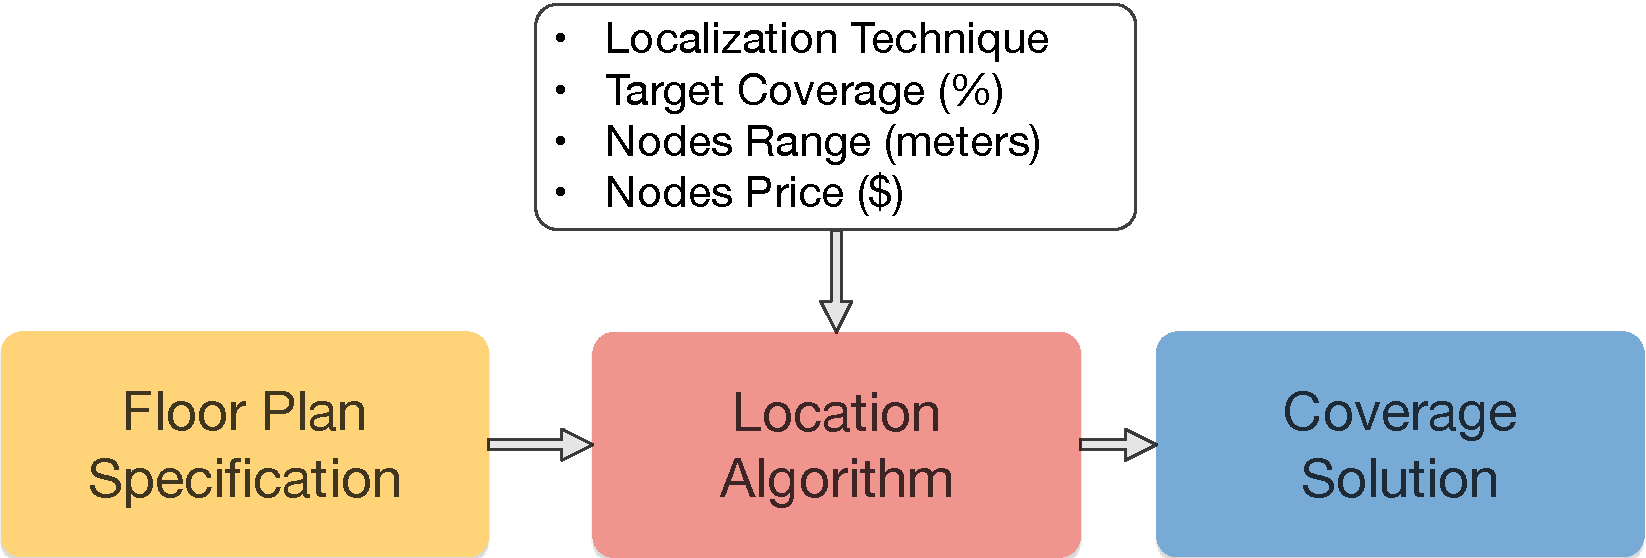
\includegraphics[width=\linewidth]{main.pdf}
\caption[System process of the CAD deployment tool for indoor WSNs.]{System Process. After the design of the floor plan, different parameters are used to define the search for an optimal allocation of nodes.}
\label{fig:main}
\end{figure}


\subsection{Covering Techniques}
\label{subsec:covering}
Our tool provides three different ways to cover the floor-plan space, each one identified by the technique required by the system that will be installed.
\begin{enumerate}[label=\textbf{(\arabic*)}]
\item \textbf{Single coverage}, that guarantees from each position the presence of at least one reachable node. This is used for example to detect the presence of a mobile device in a proximity region. In our model, a location \(l\) of the floor-plan is considered covered if exists at least one working node \(n\) of type \(t\) within a range \(r_t\). An example is shown in Fig.~\ref{fig:coverage}.a.
\item \textbf{Trilateration} is the process of determining the position of a point measuring its distance from three reference nodes, exploiting geometric properties of triangles. Usually, indoor trilateration systems use the strength of the signal received from a node to estimate its distance. In our model, a location \(l\) of the floor-plan is covered for trilateration if there exist at least three working nodes \(n_1, n_2, n_3\), each one no more distant then its corresponding range \(r_t\). A location $l$ served for trilateration is shown in Fig.~\ref{fig:coverage}.b. Although we refer only to trilateration, the same exact result can be used also for triangulation, the technique where angles are measured instead of distances.
\item \textbf{Fingerprinting}: this technique is used to estimate the position of a mobile device based on its received signal strength ($rss$) vector. Each location receives the signal from \(k\) nodes, where \(k\) is not the same for all locations, but depends on how many nodes are reachable from that particular location. Each one of the \(k\) signals reaches the receiving antenna with a given power (or $rss$). For example, the location $l$ shown in Fig.~\ref{fig:coverage}.c perceives $k=2$ signals so that $rss_{l,1} < rss_{l,2}$. We denote as \(rss_{l,n}\) the signal strength received at location \(l\) from a node \(n\). The vector \(\vec{rss_l} = [rss_{l,1}, ..., rss_{l,k}]\) of the \(k\) signals received at run-time in location $l$ is compared with a dataset of vectors, each one pre-labelled with the corresponding position.
\end{enumerate}

\begin{figure}[h!tb]
\centering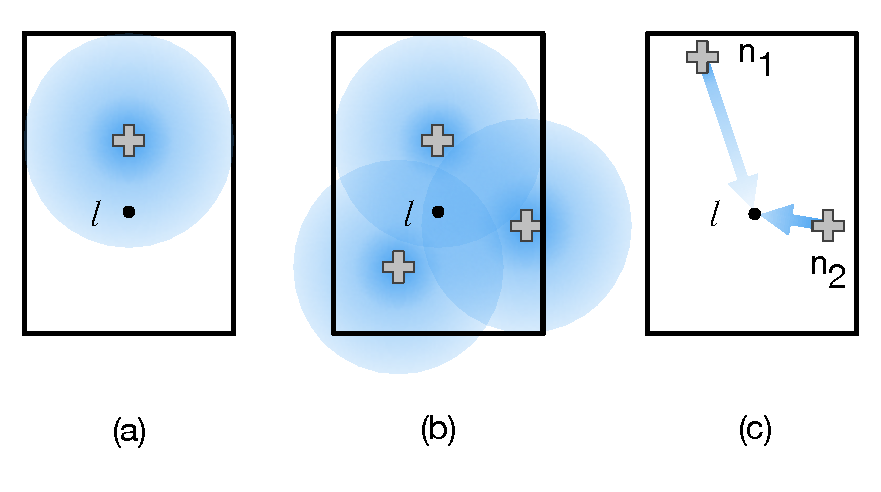
\includegraphics[scale=0.67]{coverage.pdf}
\caption[Example of indoor location covered in single, trilateration and fingerprinting mode.]{Sample floor-plans with a location $l$ covered (a) in single mode, (b) for trilateration, and (c) for fingerprinting where $rss_{l,1} < rss_{l,2}$.}
\label{fig:coverage}
\end{figure}

The comparison is usually performed by a classification algorithm using the Euclidean distance of the vectors, since $rss$ vectors with a small Euclidean distance between them are more likely to be close also in the physical space. We have defined as \(rss_{l,n}\) the signal strength received at location \(l\) from a node $n$. The Euclidean distance between $\vec{rss_a}$ and $\vec{rss_b}$, both composed by \(k\) received signals, and collected respectively in location \(a\) and \(b\) is defined as:

\begin{equation}\label{eq:E}
E(a,b)=\sqrt{(rss_{a,1} - rss_{b,1})^2 + ... + (rss_{a,k} - rss_{b,k})^2}
\end{equation}

Consider the vector $\vec{rss_a}$ as the run-time sample, while the vector $\vec{rss_b}$ retrieved from the stored fingerprint. The smaller is the \(E(a,b)\), more confident is the localization system approximating current location of \(a\) with the stored location of \(b\).

\begin{figure}
\centering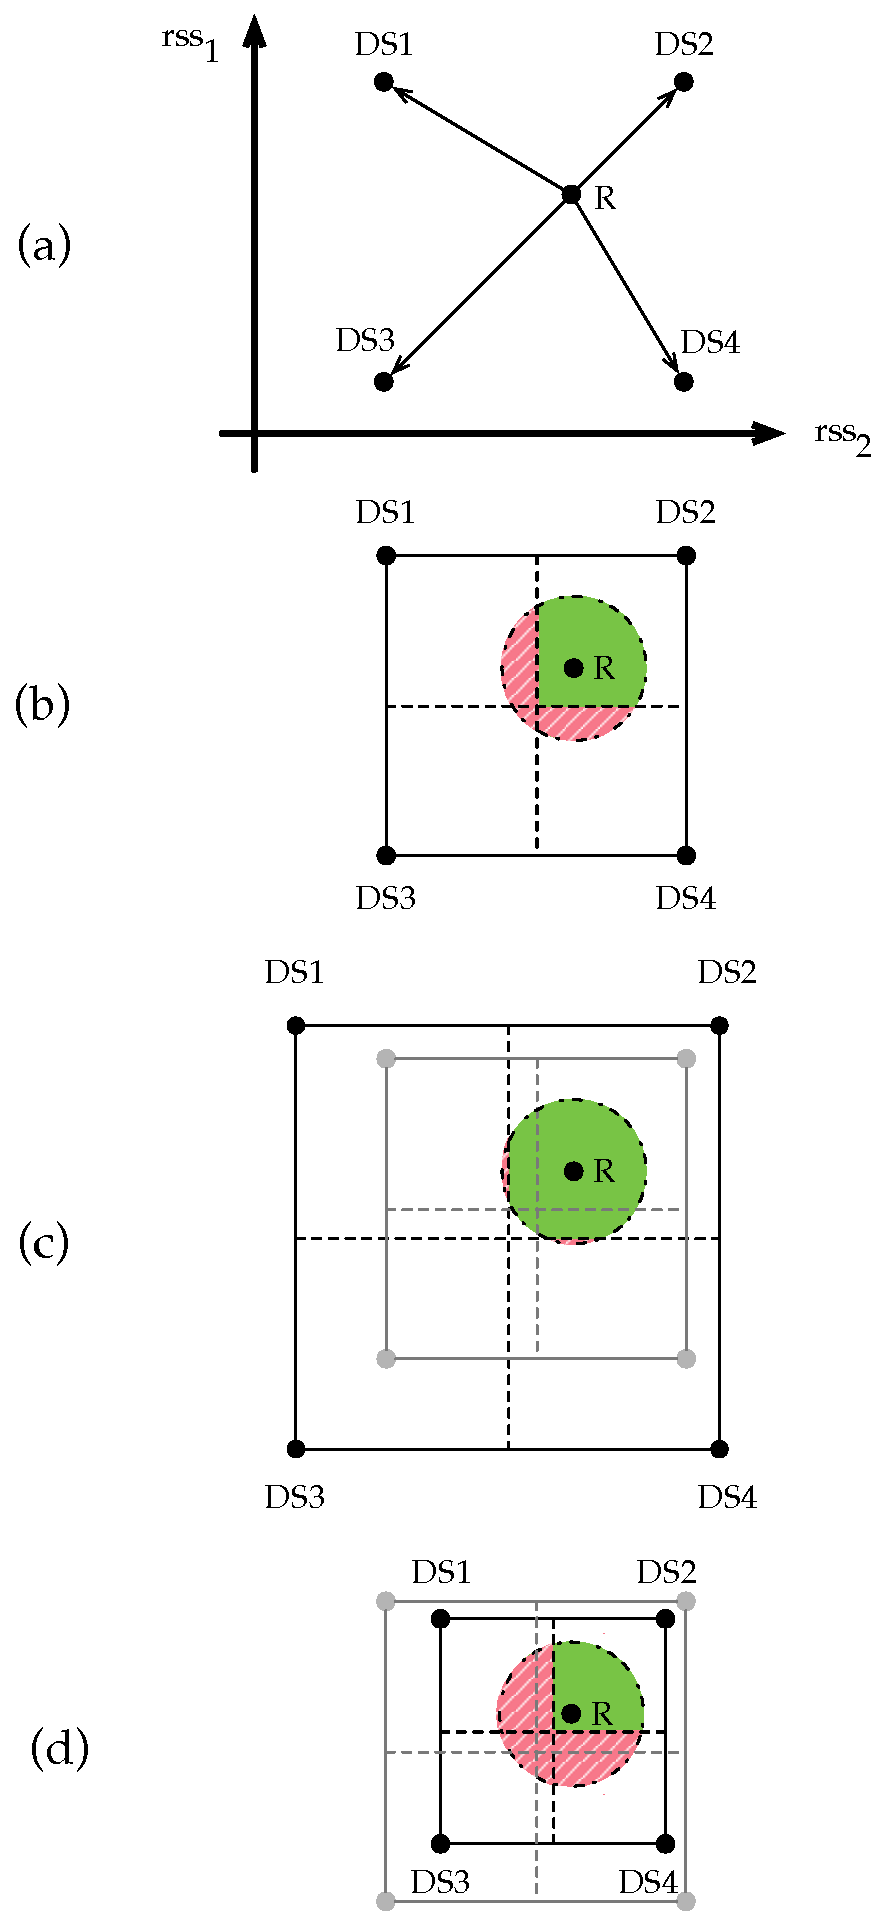
\includegraphics[scale=0.51]{example.pdf}
\caption[Relation between localization accuracy and RSS samples Euclidean distance.]{In diagram (a) bi-dimensional elements of the localization dataset are represented in Cartesian coordinates corresponding to components $rss_1, rss_2$. A run-time sample $R$ is showed in (b) where its circular area delineates signal fluctuations. Green area is proportional to the probability of correct localization, while red dashed area represent wrong localizations. In diagram (c) the Euclidean distance has been increased, thus improving the correct localization; diagram (d) shows the opposite effect.}
\label{fig:fing_example}
\end{figure}

It has been demonstrated that maximizing the Euclidean distances of the $rss$ arrays between all sampling points, the positioning accuracy of wireless localization systems can be improved \cite{Zhao2008, He2011}.
In Figure~\ref{fig:fing_example} is reported a graphical demonstration of the aforementioned statement. Take as an example a dataset ($DS1, DS2, DS3, DS4$) of stored $\vec{rss}$ vectors, where each vector is bi-dimensional ($K=2$) and coupled with the corresponding physical position. Fig.~\ref{fig:fing_example}.a shows each element of the database where the Cartesian coordinates corresponds to components $rss_1, rss_2$. Although the plane does not represent the physical area of the floor-plan, database elements that are near between them are more likely to be close also in the physical space. Given a run-time element $R$, each arrow represents the Euclidean distance $E(R,DS_i)$ from the surrounding dataset elements. A localization algorithm can exploit the Nearest Neighbor technique to approximate the position of $R$ with the nearest dataset element. Unfortunately, the run-time $rss$ measurement of $R$ will not be constant over time, but will experience continuous fluctuations due to environmental noise. These fluctuations make the sample $R$ move randomly to the surrounding points. Suppose that $DS2$ is the nearest points to $R$ in the physical space. Fig.~\ref{fig:fing_example}.b shows with a green area the probability to assign $R$ the correct (or more accurate) position, while a red (with line pattern) area represents the probability to get a wrong position from the system. Fig.~\ref{fig:fing_example}.c demonstrates how an increase in the $rss$ Euclidean distance between sampling points increase the red area and the accuracy of the localization, while in Fig.~\ref{fig:fing_example}.d an Euclidean distance reduction will lead to poorer localizations.\\



The received signal strength has been estimated using the The WINNER II path loss model \cite{Kyosti2008}:

\begin{equation}\label{eq:rss}
PL = A ~ \log_{10} (d[m]) + B + C \log_{10} (\frac{f_c [GHz]}{5.0}) + X
\end{equation}

%--------Nel caso differenziare LOS e NLOS con disegno---------

where \(PL\) is the signal path loss (in dB), \(f_c\) is the frequency in GHz, \(d\) is the distance between the transmitter and the receiver location in meters. Values of coefficients $A$, $B$, $C$, $X$ change depending on LOS (Line-Of-Sight) or NLOS (Non-Line-Of-Sight) propagations, and are reported in table \ref{tab:pathloss}. The propagation model has been used in fingerprinting coverage to maximize the Euclidean distance of the $rss$ vectors between a location and its surrounding points, with the aim of improve the localization accuracy of the system.

\begin{table}[h!tb]
\centering
\caption[Values of coefficients depending on LOS (Line-Of-Sight) or NLOS (Non-Line-Of-Sight) propagations.]{Values of coefficients depending on LOS (Line-Of-Sight) or NLOS (Non-Line-Of-Sight) propagations. Values have been taken from the WINNER II path loss model \cite{Kyosti2008}.}
\label{tab:pathloss}
\def\arraystretch{1.3}
\begin{tabular}{ | l | l |}
    \hline
    \multicolumn{1}{|c|}{\bfseries Scenario} & \multicolumn{1}{c|}{\bfseries Path Loss Coefficients} \\ \hline
    $LOS$ & $A=18.7, B=46.8, C=20$ \\ \hline
    $NLOS$ & \pbox{5cm}{
              $A=36.8, B=43.8, C=20$ \\
              $X=5(n_w-1)$ (light walls)\\
              $X=12(n_w-1)$ (heavy walls)
              } \\
    \hline
    \end{tabular}
    \end{table}

The two-dimensional space of the floor plan is discretized with a length unit (default is 1\(m\)) that is chosen by the user during the map specification phase.\\
As we have said, in addition to location coverage, also nodes connectivity has been modeled. In our model, a sensor node $n$ is connected if exist a connected path to the gateway node. To ensure the connectivity of the whole network, the following equation must hold.

\begin{equation}\label{eq:all_conn}
\forall n \in N, connected(n, gateway) = true 
\end{equation}
where
\begin{equation}\label{eq:connected}
\begin{gathered}
connected(n,n') \stackrel{def}{=} |(n,n')| \leq min(h,h')\\
\lor ~ \exists ~ n_1, \dots, n_i \in N ~ (1 < i),\\
|(n,n_1)| \leq min(h,h_1)\\
\land ~ |(n_1,n_2)| \leq min(h_1,h_2) ~\land ~ \dots\\
\lor ~ |(n_i,n')| \leq min(h_i, h')
\end{gathered}
\end{equation}

Connected networks are managed by our allocation algorithm in the same way of non-connected networks, with the following exception:
\begin{itemize}
\item first, a manual gateway nodes allocation is required;
\item during nodes allocation, deployable points $J$ are restricted to locations $j'$ such that \(connected(n_{j'}, gateway) = true\);
\item during deployment optimization, nodes moves are considered feasible only within the connected area.
\end{itemize}

\begin{table}
\centering
\label{tab:notation}
\caption{Notation and meaning of symbols used for the model.}
\begin{tabular}{ | l | l |}
    \hline
    \multicolumn{1}{|c|}{\bfseries Notation} & \multicolumn{1}{c|}{\bfseries Meaning} \\ \hline
    $L$ & set of monitoring locations \\ \hline
    $J$ & set of deployable locations \\ \hline
    $c_t$ & cost of a node of type $t$ \\ \hline
    $r_t$ & sensing range of a node of type $t$ \\ \hline
    $h_t$ & communication range of a node of type $t$ \\ \hline
    $target$ & coverage rate of $L$ required by user (\%) \\ \hline
    $n_{jt}$ & nodes of type $t$ allocated in $j$ \\ \hline
    $rss_{l,n}$ & signal strength received in $l$ from $n$ \\ \hline
    $\vec{rss_a}$ & vector of all the $rss_{a,n}$ values collected in $a$ \\ \hline
    $E(a,b)$ & Euclidean distance between $\vec{rss_a}$ and $\vec{rss_b}$\\ \hline
    $D_l$ & set of locations no more distant than $d$ from $l$ \\ \hline
    $z$ & average signal space Euclidean distance \\ \hline
    $Z$ & objective function\\ \hline
    $b_l$ & reward earned for covering location $l$\\ \hline
    $w_l$ & reward weighted on the node cost\\ \hline
    $x_{jt}$ & allocation of node with type $t$ in $j$ (binary) \\ \hline
    $a_{ljt}$ & reachability of $n_{jt}$ from location $l$ (binary) \\ \hline
    $k$-coverage & number of reference nodes required by the system \\ \hline
    $k_l$ & current number of reference nodes covering $l$\\ \hline
    $S$ & minimum signal space Euclidean distance threshold \\ \hline
    $s_{min}$ & minimum number of node moves in \emph{shaking} procedure\\ \hline
    $s_{max}$ & maximum number of node moves in \emph{shaking} procedure\\ \hline
    $Rmax$ & number of restarts of the \emph{VNS} algorithm\\ \hline


    \end{tabular}
\end{table}

\section{Covering Location Algorithm}\label{subsec:placing}
The covering location algorithm has the purpose of placing an optimal set of nodes on the building floor plan. We have decided to implement a modified version of the Multimode Covering Location Problem \cite{Colombo2016}, a generalization of the MCLP. Using a quite general and flexible reformulation of the covering problem, we have been able to adapt the algorithm at the different covering techniques described previously.

The positioning algorithm is composed by a first \emph{Greedy} procedure, whose solution is then improved by a \emph{Variable Neighborhood Search} (VNS) algorithm.
The positioning algorithm evaluates different solutions using a reward \(b_l\), that is defined for each location $l$ and will be earned only for the locations covered in that particular solution. The value of the reward depends on the coverage technique:

\begin{itemize}
\item Single coverage: the reward \(b_l\) will be earned if there is at least one node that covers $l$.
\item Trilateration: the reward \(b_l\) will be earned if there are at least three nodes that cover $l$.
\item Fingerprinting: since this technique is often considered to be a trade-off (in cost and accuracy) between single coverage and trilateration, we decided that the reward \(b_l\) will be earned if there are at least two nodes that covers $l$.
\end{itemize}

%--------- distanza euclidea dai surrounding locations ----------
As we have said, in order to maximize the localization accuracy of the system it's possible to increase the signal space Euclidean distance between the target points.
Consider the mean Euclidean distance between the received $rss$ vector in a certain location \(l\), and the surrounding locations $s$ within a certain distance \(d\):
\begin{equation}\label{eq:fing}
\begin{gathered}
\frac{1}{\mid D_l \mid} \sum\limits_{s \in D_l} E(l,s)\\
D_l = \{s \in L \mid distance(l,s)  \leq d\}
\end{gathered}
\end{equation}
The distance $d$ is used to restrict the $rss$ comparison and diversification only to the locations that are more likely to be erroneously confuse with $l$ by the localization system. Fig.~\ref{fig:rssdiv} shows an example of how the Euclidean distance of a location is compared to a neighbor location.


\begin{figure}
\centering
\begin{minipage}{0.63\textwidth}

\begin{equation}
\begin{gathered}
\nonumber
\vec{rss_l} = \langle rss_{l,1}, rss_{l,2} \rangle = \langle-84, -72\rangle ~ [dB] \\
\vec{rss_s} = \langle rss_{s,1}, rss_{s,2} \rangle = \langle-67, -41\rangle ~ [dB] \\[5pt]
E(l,s) = \\ = \sqrt{(rss_{l,1} - rss_{s,1})^2 + (rss_{l,2} - rss_{s,2})^2} = \\
= \sqrt{(-84-(-67))^2 + (-72-(-41))^2} = \\ = 35.3 ~ [dB]
\end{gathered}
\end{equation}

\end{minipage}%%%
\begin{minipage}{0.37\textwidth}
\centering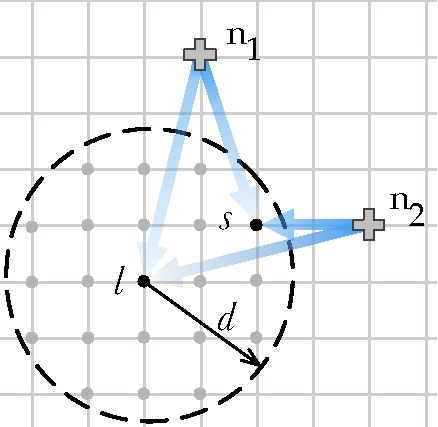
\includegraphics[width=\linewidth]{rssdiv.pdf}
\end{minipage}
\caption{Regular grid showing how is computed the mean Euclidean distance between the received $rss$ vectors in a certain location \(l\), and the surrounding locations $s$ within a certain distance \(d\).}
\label{fig:rssdiv}
\end{figure}

We define the average signal space Euclidean distance $z$:
\begin{equation}\label{eq:z1}
z = \frac{ \sum\limits_{l \in L} \sum\limits_{s \in D_l}\frac{E(l,s)}{|D_l|}}{|L|}
\end{equation}

The term $z$ will be used by the \emph{Greedy} procedure to produce a first solution with a reasonable allocation of nodes. Then, the value of $z$ should be increased as much as possible to provide good localization accuracy to the system. However, maximize only the average does not seems fair enough, since a good system should provide a certain level of accuracy homogeneously among the target area. So we defined the objective function as difference between the term $z$ and the signal space Euclidean variance:

\begin{equation}\label{eq:Z1}
Z = z - \sqrt{\sum\limits_{l\in L}\left(\sum\limits_{s\in D_l}\frac{E(l,s)}{\mid D_l \mid}\right)^2}
\end{equation}

Maximizing the objective function $Z$, the intention is to provide as many target location as possible with a high signal space Euclidean distance with respect to the surrounding locations.


As we have previously introduced, we represent with \(L\)  the entire set of location to be covered, while with \(J\) the set of possible positions where nodes can be placed. By default, \(L = J\) and nodes can be positioned everywhere; however its possible to restrict the \(J\) set only to specific candidate points, that represent for example power outlets or Ethernet sockets.
The problem of find a near-optimal set \(N\) of nodes \(n_{jt}\) (each one located in $j$ and having a type $t$) with a coverage rate $f(N)$ that satisfies the $target$ coverage, can be formalized as follows.
\begin{equation}\label{eq:Z}
\max Z = z - \sqrt{\sum\limits_{l\in L}\left(\sum\limits_{s\in D_l}\frac{E(l,s)}{\mid D_l \mid}\right)^2}
\end{equation}
\begin{equation}\label{eq:cov}
f(N) \geq target
\end{equation}
\begin{equation}\label{eq:one}
\sum\limits_{t \in T} x_{jt} \leq 1 \quad \forall j \in J
\end{equation}
\begin{equation}\label{eq:x}
x_{jt} = 1 \quad \iff n_{jt} \in N
\end{equation}
\begin{equation}\label{eq:f}
f(N)= \lvert L \rvert / \sum\limits_{l \in L} y_l
\end{equation}
\begin{equation}\label{eq:y}
\begin{cases}
y_l \leq \sum\limits_{j \in J}\sum\limits_{t \in T} a_{ljt} x_{jt} \quad \forall l \in L ~ (single)\\
2~y_l \leq \sum\limits_{j \in J}\sum\limits_{t \in T} a_{ljt} x_{jt} \quad \forall l \in L ~ (fingerprinting)\\
3~y_l \leq \sum\limits_{j \in J}\sum\limits_{t \in T} a_{ljt} x_{jt} \quad \forall l \in L \quad (trilateration)\\
\end{cases}
\end{equation}

The decision variable $x_{jt}=1$ represents the allocation of a node of type $t$ in location $j$; $a_{ljt}$ is equal to $1$ if location $l$ can be reached by a node of type $t$ placed in $j$, and $a_{ljt}=0$ otherwise. $y_l=1$ if location $l$ is covered, $y_l=0$ otherwise. The constraint \eqref{eq:one} fixes to one the maximum number of nodes that can be located in each site.

\subsection{Greedy Procedure}\label{subsec:greedy}
The positioning algorithm starts with a \emph{Greedy} procedure with the purpose of find a reasonable number of reference nodes, for both coverage and localization accuracy. The procedure generate a first solution \(N\) positioning a set of \(k\) = $\lvert N \rvert$ nodes, each one with a type \(t \in T\).
For all three coverage techniques, the reward $b_l$ is weighted with the cost of the current node $n^*$ selected for the coverage:
\begin{equation}\label{eq:w}
w_l = \frac{b_l}{ c_t}; \quad \{n^*=n_{jt} ~ \land ~ distance(j,l)  \leq r_t\}
\end{equation}
The weighted reward $w_l$ will be used by the \emph{Greedy} algorithm so that on equal covered area, the cheapest node type has the priority over the others.
We denote as \(L_{jt}\) the subset of locations that are reachable by a reference node \(n\) of type \(t\) placed at location \(j\). At each iteration, the algorithm places a node \(n\) of type \(t^*\) at position \(j^*\) that covers the subset of locations \(L_{j^*t^*}\) with the maximum reward. The term
\begin{equation}\label{eq:kcov}
1 - \frac{k_l}{k-coverage}
\end{equation}
is used to prioritize the covering of locations with a lower 'temporary' \mbox{$k$-coverage} (called $k_l$) with respect to the \mbox{$k$-coverage} required by the current techniques. In this way, \emph{Greedy} procedure tends to avoid the placement of nodes very close to one other which can lead, especially for trilateration systems, to poor localization accuracy.
It's important to notice that the purpose of the \emph{Greedy} procedure is to find a reasonable number of nodes for the localization service. The starting positioning is made on a best-effort basis, that will be improved by the successive \emph{VNS}.
After a node allocation, all subsets \(L_{jt}\) are updated according to the coverage technique. In trilateration for example, a location \(l\) is removed from \(L_{jt}\) only if there exist, other than the current  \(n_{j^*t^*}\), other two nodes that are already covering \(l\).

\begin{algorithm}
\caption{\(Greedy(L, J, T, w, target)\)}
\begin{algorithmic}%[1] row numbers
%\Procedure{MyProcedure}{}
\label{alg:greedy}
\State $N := \varnothing$;
\State $L_{jt} := \{l \in L \mid l$ is covered by node in \(j\) with type \(t\)\};
\While{$(f(N) < target) \land (z < S)$}
\State $j^{*} := \argmax{j \in J} \sum\limits_{l \in L_{jt}}w_l ~ (1 - \frac{k_l}{k-coverage})$;
\State $t^{*} := \argmax{t \in T} \sum\limits_{l \in L_{jt}}w_l ~ (1 - \frac{k_l}{k-coverage})$;
\State $N := N \cup \{n_{j^*t^*}\}$;
\State $L_{jt} := L_{jt} \setminus L_{j^*t}$ for all $j \in J$;
%\State update $coverage$;
\EndWhile
\State \Return $N$;
%\EndProcedure
\end{algorithmic}
\end{algorithm}

The \emph{Greedy} procedure ends when the $target$ coverage is satisfied, and when the average signal space Euclidean distance $z$ reaches the threshold $S$. In our implementation we set the threshold $S=4.5$ that has been proven to be the average Euclidean distance for which the positioning error is limited to 2 meters \cite{He2011}.
How we will see in the {\hyperref[cap:results]{experimental results chapter}}, the \emph{Greedy} procedure is able to provide an average Euclidean distance not so far from the final best known. However, thanks to the low complexity of the \emph{Greedy} procedure, additional time can be used to improve the solution. In addition, the Euclidean distance variance will be strongly improved.

\subsection{Variable Neighborhood Search}
The method called \emph{Variable Neighborhood Search} (VNS) has been used to improve the solution coming from the \emph{Greedy} procedure. The VNS approach empowers the classical local search framework with a restart mechanism that extends the search after a local optimum has been achieved by generating new starting solutions in progressively enlarged neighborhoods of the current best known solution. The key elements of the VNS (reported in algorithm 2) are a starting solution $N$ with a hierarchy of size-increasing neighborhoods, and a local search procedure, i.e., the criterion to select the incumbent solution from the neighborhood. These components are used to restart the search every time that the procedure reaches a local optimum.
Figure~\ref{fig:algorithm} shows an overview of the VNS process. 
\begin{figure}[h!tb]
\centering\includegraphics[scale=0.25]{algorithm.pdf}
\caption{Location Algorithm. The solution found by the \emph{Greedy} algorithm is improved applying iteratively a \emph{Local Search} for an optimal solution and a \emph{Shaking} procedure that perturbs the current solution.}
\label{fig:algorithm}
\end{figure}
A first local search procedure is applied to the solution produced by the \emph{Greedy} procedure. At each iteration, the \emph{shaking} procedure is used to generate a new starting solution, which is then improved by the execution of the local search. The shaking procedure perturbs \(s\) node allocations of the current solution \(N^*\) replacing them with \(s\) unused nodes. The behavior of the shaking parameter \(s\), that depends on the result of the local search, is explained in Figure~\ref{fig:shaking}. 
\begin{figure}[h!tb]
\centering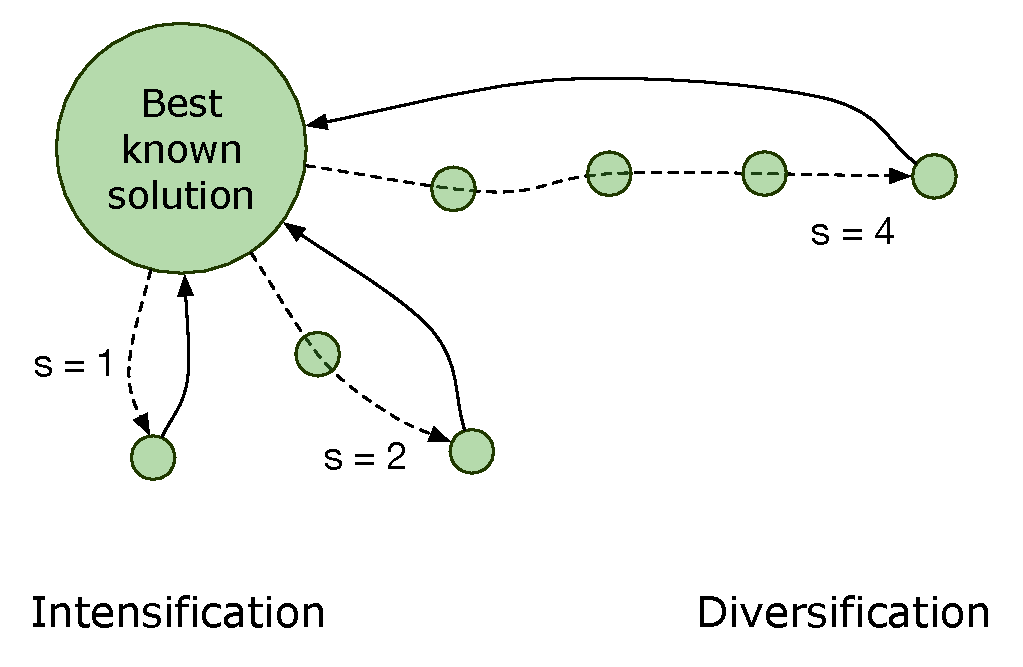
\includegraphics[scale=0.55]{VNSgraph.pdf}
\caption{Shaking procedure: the parameter $s$ is increased when the solution does not improve (dashed line) and restarts when a new optimum is found (continuous line).}
\label{fig:shaking}
\end{figure}
The parameter \(s\) starts from a minimum value \(s_{min}\) (in the example \(s_{min} = 1 \)) and every time that the local search does not improve the best known solution, \(s\) is increased by 1. Differently, when the local search succeeds, the best solution \(N^*\) is updated and \(s\) goes back to \(s_{min}\).

The purpose of the shaking procedure is to first explore new starting solutions that are more similar to the best known result, so that the search is \emph{intensified} in a promising neighborhood of the entire domain. If these local searches fail, the shaking procedure moves the search from intensification to \emph{diversification}, generating starting solutions that are more and more different from the incumbent one. Whenever a new best solution is found, the shaking procedure comes back to \(s_{min}\), to intensify the search near the just updated \(N^*\). In principle, the shaking parameter \(s\) can be increased until $k=\lvert N^* \rvert$, changing all the node allocations. However, we experimented running different configurations that excessively moving away from the best known solution can be unproductive, causing a useless waste of computational time. We have fixed a reasonable value of \(s_{max} = \floor{\frac{2}{3}k}\).

\begin{algorithm}
\caption{\(VNS (L, J, T, w, target, s_{min}, s_{max}, R_{max})\)}
\begin{algorithmic}%[1] row numbers
\label{alg:vns}
%\Procedure{MyProcedure}{}
\State $N:=Greedy(L, J, T, w, target)$;
\State $N^{0}:=LocalSearch(L, J, T, w, target)$;
\State $N^* := N^0$;
\State $s := s_{min}$;
\For{$r:=1$ to $R_{max}$}
\State $N:= Shaking(N^*, s, L, J, T, w, target)$
\State $N^0:= LocalSearch(L, J, T, w, target)$
\If{($Z(N^0) > Z(N^*)$)}
\State $s:=s_{min}$;
\State $N^*:=N^0$;
\Else
\State $s:=s+1$;
\If{($s > s_{max}$)}
\State $s:=s_{min}$;
\EndIf
\EndIf
\EndFor
\State \Return $N^*$;
%\EndProcedure
\end{algorithmic}
\end{algorithm}

The VNS algorithm terminates when the total number of restarts reaches a given value $R_{max}$.
%In our implementation, we have decided to make the value of $R_{max}$ vary adaptively, depending on the size of the problem instance ($\lvert J \rvert$, $\lvert T \rvert$). 

As we have said, the local search is the heuristic that proceeds from an initial solution to its neighborhood by a sequence of local changes, trying to improve each time the value of the objective function until a local optimum is found.
The neighborhood of the adopted approach is given by cyclic sequences of moves, where each move consists in locating a new node, removing a node or changing the type of the node. A cyclic move is considered feasible only if the new covering rate respects the \emph{target} coverage, and the total cost of the solution does not increase. Of course, each site must continue to hosts at maximum one node (constraint equation \eqref{eq:one}). A cyclic move can be visualized on a graph $G=(N,A)$, where each node of the graph is a possible allocation of a hardware node. Each node of the graph is characterized by a location $j$, and a state that indicates if the node is active or inactive. A node $n_{jt}$ currently allocated in location $j$, is represented on the graph with an active node $n_j$, labeled with its hardware type $t$. Note that index $t$ does not appear because at most one type can be active in each node, and the type is specified by the label. Inactive nodes are instead left unlabeled. An arc ($n_j, n_k$) can represent:
\begin{enumerate*}[label={(\arabic*)}]
\item the allocation of a hardware node in site $j$, if $n_j$ is inactive and $n_k$ is active;
\item the removal of a hardware node in site $j$, if $n_j$ is active and $n_k$ is inactive;
\item an hardware node $n_j$ changing its hardware type, if both nodes are active.
\end{enumerate*}
In both (1) and (2), the new node takes the hardware type of the head label ($t$ of $n_k$). A cyclic exchange corresponds to a directed cycle on the improvement graph, as depicted in Figure~\ref{fig:graph}. 
\begin{figure}[h!tb]
\centering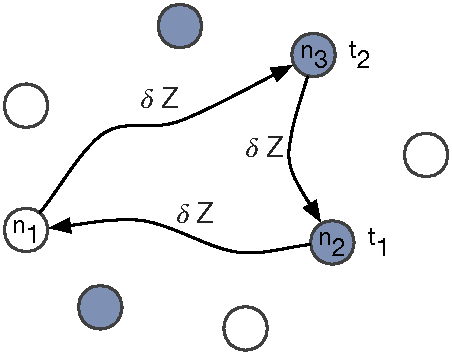
\includegraphics[scale=0.7]{graph.pdf}
\caption{Improvement Graph: colored nodes represent current allocations, while empty nodes are possible allocations. All active nodes are labeled with their corresponding type. Each arc is a change (move) on the allocations.}
\label{fig:graph}
\end{figure}
Each move, and so each arc ($n_j, n_k$), determines a variation $\delta Z$ in the value of the objective function $Z$. The purpose is to represent a group of moves so that a cyclic exchange represents an increase in the current objective function. However the total variation $\delta Z$ is non additive with respect to the sequence of $\delta Z$ values coming from single moves. This is caused by the interdependence between different hardware nodes with overlapping covering regions, that lead to non-additive moves. To overcome this drawback, every cycle has been evaluated using an own temporary function $Z'$ updated step by step from the end of the path to its starting node. In this way, all the cycles with a positive total weight bring improvements on the starting solution.

The search for the cyclic exchange with maximum weight is performed with exhaustive breadth-first exploration of the paths of graph $G$.


%\section{Experimental Results}\label{sec:results}

% \section{Limitations, future works and Conclusions}
% A first limitation of the proposed approach reside in the propagation model used to compute near-optimal solutions for localization systems. The model implemented is site-specific, and take in consideration walls for LOS and NLOS propagations. However the approach do not consider refraction or diffraction effects. Another limitation is the inability of the system to model the signal propagation between different floors of the building, managing each level independently.\\
% For future work, we plan to improve the system with an indoor signal propagation model able to consider refraction and diffraction effects of the indoor environment like walls and floors. In addition, we'll try to apply the model to 3D designing tools, becoming suitable also for multi-floor environments.
%This model keep into account a floor penetration loss factor, becoming applicable also for multi-floor environments.


\section{Conclusions and Future Work}
In this chapter, we tried to explain the challenges faced by designers during the installation of smart building systems that require the positioning of several hardware nodes. A common limitation of existing models is the lack of a convenient way to specify geometric information of the indoor map. This also leads to the employment of less accurate general models for signal propagation, instead of site-specific models. The design phase is get more difficult by the availability on the market of different hardware nodes, with different power transmissions and costs.

For these reasons we propose an integrated tool for both floor plan specification and node positioning, developed within an \mbox{open-source} CAD environment extensible through plug-ins. The tool is able to provide a near-optimal solution of node allocations, possibly with mixed types, with the aim to reduce the installation costs. The results suggest that, for most of the problem instances, a solution can be obtained in a reasonable execution time. Depending on the available hardware types, total cost of the solution could be improved moving from homogeneous to mixed type allocation.

A limitation of the proposed approach resides in the propagation model used to compute near-optimal solutions for localization systems. The model implemented is site-specific, and take in consideration walls for LOS and NLOS propagations. However the approach do not consider refraction or diffraction effects. Another limitation is the inability of the system to model the signal propagation between different floors of the building, managing each level independently.
For future work, we plan to improve the system with an indoor signal propagation model able to consider refraction and diffraction effects of the indoor environment like walls and floors. In addition, we'll try to apply the model to 3D designing tools, becoming suitable also for multi-floor environments.